\newpage
\sect{Appendix E \quad Retrospective batch scheduling with local supervision}
An updated edge classifier can change both its answers and the order in which it asks for help. We gave every strategy the same ceiling in application bytes. A review transmits a real 224-pixel JPEG and 20 bytes of request and reply fields to the same frozen PlantDoc-balanced DINO service. Unqueried images keep their edge decisions. The original camera queues frames closest to its released 0.30 cutoff. The updated camera queues frames with the smallest absolute distance from its new logit cutoff of zero. The sender knows JPEG lengths after encoding and can buffer the batch. A frame is skipped if it does not fit in the remaining allowance. The scheduler sees no evaluation label or remote prediction before making that choice.

For this historical batch comparison we fixed a ceiling of 25\% of the bytes for full review, with 10\% and 50\% for sensitivity. The 20 Cornell-trained 128-label heads in Appendix~B are reused without refitting. We charge the complete calibration and deployment cost to each cohort, including both transfers. If an update cannot fit, the combined system uses the original edge router. The table assumes the 128 reference labels are available at the camera during Cornell calibration.

\begin{center}\small
\begin{tabular}{@{}lrrr@{}}\toprule
Mean BA (\%), 25\% ceiling unless marked & Cornell & Kashmir & Latvia\\\midrule
Frozen server on every image (100\% ceiling) &83.56&83.40&60.64\\
Original edge &69.74&67.58&46.90\\
Original edge + selective review &72.62&76.37&51.54\\
Updated edge alone &80.01&78.91&52.11\\
Updated edge + random review &80.85&79.75&54.55\\
Updated edge + selective review &\textbf{87.06}&\textbf{84.28}&\textbf{54.74}\\\bottomrule
\end{tabular}\end{center}
\note{Latvia uses the presence of visible scab as its endpoint. The random control uses 20 fixed image orderings for each of the 20 head draws and pays the same setup cost. Selective review used means of 283, 75 and 272 uploads (rounded).}

\begin{center}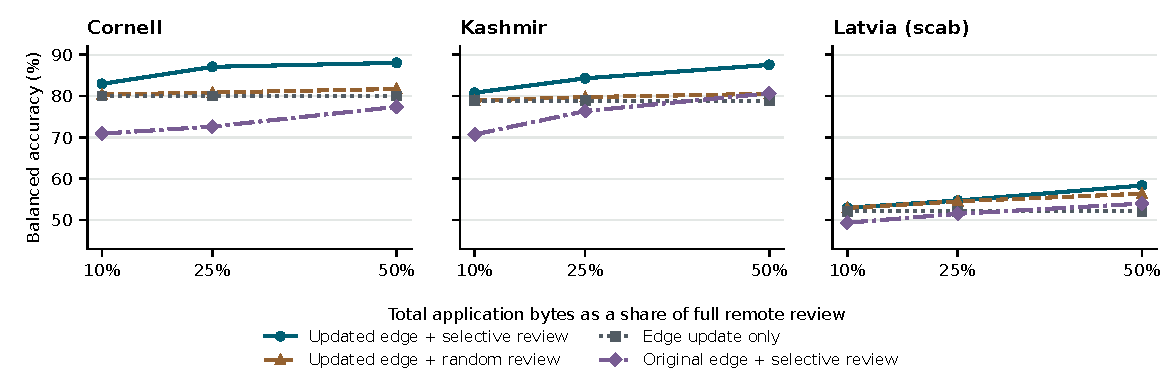
\includegraphics[width=.96\linewidth]{figures/collaboration.pdf}\end{center}
\note{Figure E1. Each cohort uses its own byte ceiling. Each mean reuses a single evaluation pool across draws. The line for the update alone falls back to the original camera if the update cannot fit.}

On Cornell and Kashmir, every calibration draw beat both single interventions at 25\%. The selective policy corrected 100.45 and spoiled 33.35 Cornell decisions per draw, compared with the updated edge alone. On Kashmir these values were 24.65 and 8.20. On Latvia the selective and random policies were within 0.19 points, and only 10 of 20 draws beat mean random review. The service corrected 51.45 decisions and spoiled 91.55 on average there. With 207 negatives and 983 positives there, ordinary accuracy fell from 73.70\% for the original camera to 48.67\% for the joint policy. Mean scab misses rose from 118 to 536.35.

If the Cornell calibration photographs must be transmitted for annotation, joint BA at 25\% becomes 84.76\%, 76.37\% and 53.70\%, respectively. On Kashmir the mean calibration exchange alone exceeded the entire 945,647-byte allowance in every draw. Paying for the labels eliminates the update at this ceiling.

\newpage
\sect{Appendix F \quad Can full review reduce false alarms and misses together?}
Changing one cutoff on a fixed ordering adds or removes alerts in a single direction. To examine two independent changes, we allowed the source-balanced remote model to rescue an edge-negative image and to retract an edge-positive alert. A 475-rule grid was fixed before examining results for this policy. We used the 450 Cornell calibration images to require at least a halving of the 15 original misses and fewer than the 83 original false positives. Four rules qualified. Prespecified tie-breaking first minimized false positives. The selected rule yielded 60 false positives and five misses on calibration. Earlier methods had already been evaluated on the Cornell and Kashmir test collections.

The selected rule queried every photograph. For an original negative it issues an alert if the service's estimated disease probability is at least 0.50. For an original positive it clears the alert only below 0.30. Fitting required 3,031,861 calibration bytes, followed by a 22-byte configuration. All deployments below replay the very same configuration.

\begin{center}\small
\begin{tabular}{@{}lrrr@{}}\toprule
Source and reference counts & False positives & False negatives & Inference bytes\\\midrule
Cornell (377 negative, 976 positive) &$215\to137$&$34\to19$&9,141,584\\
Kashmir (128 negative, 256 positive) &$81\to25$&$4\to25$&3,782,589\\
Latvia (207 negative, 983 positive) &$195\to83$&$118\to334$&10,788,080\\\bottomrule
\end{tabular}\end{center}

The Cornell rule corrected 108 false alarms and 25 missed cases, while introducing 30 false alarms and 10 misses. Much of its net rescue came from scab, where misses fell from 21 to four. Among 67 images with multiple diseases, misses increased from one to four. In Kashmir, 22 of the 24 introduced misses occurred on Alternaria. Only three originally missed Kashmir cases were rescued. These counts come from the same image decisions and distinguish the type of mistake that moved the average.

\subt{Competing choices of representation and operating point}
On Cornell, a single 448-pixel JPEG with three DINO views, fitted on 300 Cornell examples and thresholded on the remaining 150 calibration examples, yielded 83 false positives and 38 misses at a cost of 26,528,371 inference JPEG bytes. On Kashmir it yielded four and 75 respectively. On Latvia it yielded 37 and 401. A preselected two-score fusion yielded 120/39, 22/33 and 64/404, respectively (false positives/misses). Using more pixels or adding two scores can suppress false alarms while losing the intended sensitivity.

Two of 20 earlier high-sensitivity INT8 heads (draws 2 and 4) reduced both counts on both Cornell and Kashmir. They were identified after examining those results. Both were then fixed for Latvia, where their error counts were 192/126 and 181/164, respectively, against the original 195/118. Conditional selection would have overstated their portability.

A stronger single-expert control received the identical 450 labels and considered every distinct observed remote-score cutoff and its endpoints. Under the common calibration constraint of at most seven misses it selected 0.33966 (63 false positives and five misses). In full review it gave 173/18 on Cornell, 25/34 on Kashmir and 62/359 on Latvia. Against this control, the directional combination eliminated nine further misses at unchanged false positives on Kashmir. In Latvia it exchanged 21 additional false positives for 25 fewer misses. The fixed 0.50 remote model also retained higher Cornell BA than the directional combination (83.56\% versus 80.86\%). Threshold comparisons and both single-score controls are included in the artifact. The two-score rule's value depends on the cost assigned to each error.


\newpage
\sect{Appendix G \quad External scab screening and local recalibration}
AppleScabLDs contains all 1,190 leaf photographs in the specified Latvian archive \cite{kodors}, with 207 publisher-negative and 983 visible-scab references. An image without visible scab can show other damage. Photographs include repeated leaf views. An independent ZIP traversal verified all paths, SHA-256 values, labels and perceptual hashes. No exact or perceptual match within Hamming distance five was found against 7,575 archived source images. In the Latvian archive, one member per same-label component at distance four yields 1,148 representatives. The fixed Cornell rule changes false positives from 191 to 81 and misses from 116 to 324 on this subset. Neither perceptual grouping nor spatially distinct collections establishes leaf-level statistical independence.

All images retained original capture dates over 14 days. We reserved the earliest five full days for calibration and all nine later days for evaluation, before looking at the new predictions. No exact or screened near-duplicate component crossed these two partitions. The five days supplied 611 images and labels, including 476 with scab. The later days contained 72 negatives and 507 positives. The date split therefore required substantially more calibration images than a one-third split of individual files.

The identical 475-rule procedure found no candidate that halved calibration misses while lowering false positives. Its prespecified fallback chose among the 38 rules that strictly lowered both. It changed early error counts from 128/69 to 126/56. On the 579 later images the baseline had 67 false positives and 49 misses. The Cornell rule yielded 30 and 159. The rule calibrated on the five local dates yielded 67 and 33. It rescued 18 missed scab images and incorrectly withdrew two true alerts. Sensitivity rose from 90.34\% to 93.49\%, while specificity remained 6.94\%. The early labels and rule installation cost 5,497,944 bytes, followed by 1,554,379 bytes for 175 later queries. This is a within-season analysis with a small later negative cohort.

\begin{center}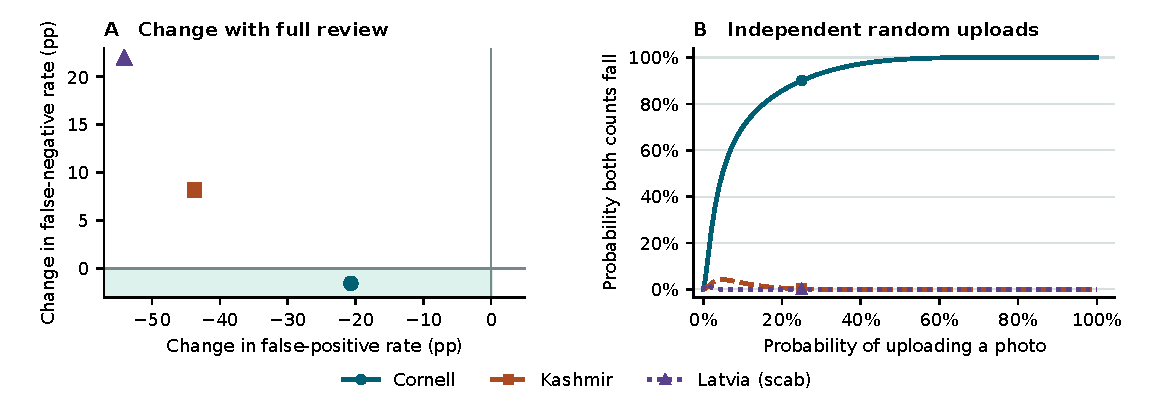
\includegraphics[width=.96\linewidth]{figures/joint_errors.pdf}\end{center}
\note{Figure G1. Left, the shaded quadrant denotes strictly fewer errors in both classes. Right, for a fixed set of scored images, the only randomness is an independent decision to upload each eligible image with probability $q$. At $q=1$ all eligible images get the full-review treatment.}

If full review fixes $a$ and spoils $b$ decisions of one true class, independently sampling eligible uploads with probability $q$ gives a strict improvement probability $P[\mathrm{Bin}(a,q)>\mathrm{Bin}(b,q)]$ for that class, using two independent binomials. The two class-specific events involve disjoint uploads, so their probabilities multiply. At $q=0.25$ the probability of a strict joint reduction is 90.05\% on the fixed Cornell batch and 0.23\% on the fixed Kashmir batch. This retrospective calculation quantifies routing randomness. It assumes no probability law for new leaves.
